\chapter{Proof of Concept}
\label{sec:proofofconcept}

% PHP/XEDUB installation: https://ubuntuforums.org/showthread.php?t=525257
%						  https://www.youtube.com/watch?v=OlcsQ8TCU3A
%	> sudo add-apt-repository ppa:ondrej/php
%	> sudo apt-get update
%	> sudo apt-get apache2
% 	> sudo apt-get install php7.1-dev php-pear php7.1-mbstring php7.1-cgi	  			// old... > sudo apt-get install php5-dev php-pear
%	> sudo apt-get install libapache2-mod-php7.0
% 	> sudo pecl install xdebug
% 	> find / -name 'xdebug.so' 2> /dev/null
% 	/usr/lib/php5/20060613/xdebug.so
% 	> sudo gedit /etc/php/7.1/apache2/php.ini		
%		[xdebug]
%		zend_extension=/usr/lib/php/20160303/xdebug.so
%		xdebug.default_enable=1
%		xdebug.idekey=PHPSTORM
%		xdebug.remote_enable=1
%		xdebug.remote_port=9000
%		xdebug.remote_connect_back=1

% Enabling error msg. Set "`display_errors = On"' in:
%	> sudo gedit /etc/php/7.1/apache2/php.ini	

% Change document root:
% 	> sudo gedit /etc/apache2/sites-available/000-default.conf
%	> sudo gedit /etc/apache2/apache2.conf
% 	> sudo /etc/init.d/apache2 restart

% Installing grunt (as npm package):
%	> npm init
%	> npm install grunt --save-dev
%	create Gruntfile and update package.json according to: https://gruntjs.com/getting-started and http://www.wearecube.ch/from-less-to-css-with-grunt-js/
%	> npm install
%	> grunt
%					// > grunt watch &				// grunt watch will be stoped when the commandline closes

% installing composer/twig:
% 	download to project root: https://getcomposer.org
% 	> php composer-setup.php --filename=composer
%	create composer.json in project root. content:
% 		{
%			"require": {
%   			"twig/twig": "1.*",
%			    "twbs/bootstrap": "3.3.7"
%  			}
%		}
%	> php composer.phar install 		or			php composer.phar update
%	> sudo chown www-data:www-data bookinganalyzerimpl/compilation_cache/

% https://nikic.github.io/2011/12/12/How-big-are-PHP-arrays-really-Hint-BIG.html
% installing redis
%	> sudo pecl install redis
%	Adding "extension=redis.so" to php.ini
%	  	> sudo gedit /etc/php/7.1/apache2/php.ini	
%	  	> sudo gedit /etc/php/7.1/cli/php.ini	
% 	> sudo /etc/init.d/apache2 restart
%
%	> wget http://download.redis.io/releases/redis-3.2.8.tar.gz
%	> tar xzf redis-3.2.8.tar.gz
%	> cd redis-3.2.8
%	> make
% 	> ~/programs/redis-3.2.8/src/redis-server
% http://www.codeforge.com/article/214557


% Getting bookinganalyzerimpl to run:
% git clone git@github.com:soultemptation/bookinganalyzerimpl.git
% npm install
% grunt
% php composer.phar install

% Remove duplicates:
%			Find duplicates:
%			> egrep -o '^[^@]+' u611a_10_normalized_geocoded.csv > text.csv 	// Get everything before first @
%			> sort text.csv > text_sorted.csv									// Sort it
%			> uniq -d text_sorted.csv > text2_duplicates.csv					// Remove duplicates
% 	> tac u611a_10_normalized_geocoded.csv | sort -k1,1 -r -u -t@ > text5.csv
%	> tac text5.csv > text6.csv
%	Move last line of text6.csv to the beginning

\section{Datenvorbereitung}
\label{sec:proofofconcept:datenvorbereitung}

% Feature selection
% https://en.wikipedia.org/wiki/Feature_selection
% http://dollar.biz.uiowa.edu/~street/research/dmoc.pdf
% http://www.jmlr.org/papers/volume3/guyon03a/guyon03a.pdf

\subsection{RapidMiner Prozess für die Datenvorbereitung}
\label{sec:konzept:rapidminer}

Die Datenvorbereitung (data preprocessing) wird mit dem Programm RapidMiner durchgeführt.
Zuerst werden die Daten aus dem \gls{csv} File geladen. Anschliessend die Attribute gemäss \cref{fig:recherche:attributeinschraenkung:2} eingeschränkt sowie die Diskretisierung entsprechend \cref{fig:recherche:datenvorbereitung:1} und \ref{fig:recherche:datenvorbereitung:2} durchgeführt.

\cref{fig:recherche:rapidminer:1} zeigt den Prozess im RapidMiner Studio. In \ref{fig:recherche:rapidminer:1:1} wird der Hauptprozess gezeigt. Zusätzlich sind die Operatoren "`Generate ID"' und "`Write CSV"' vorhanden. Ersterer generiert eine neue ID. Da im Schritt "`Select Attributes"' keine Kundenspezifischen Daten ausgewählt werden, sind die Informationen nacher voll anonymisiert und können auch veröffentlicht werden. Der letzte Schritt schreibt das Resultat in ein \gls{csv} File damit es nachher weiterverwendet werden kann.

\cref{fig:recherche:rapidminer:1:2} ist ein Unterprozess welcher die Diskretisierung des Preises und der Distanzen vornimmt. Im \cref{sec:recherche:datenvorbereitung} wird beschrieben dass nicht alle Bereich der zu diskretierenden Attribute verwendet werden soll (z.B. Distanzen >499 werden nicht berücksichtigt). Dies kann mit den "`Discretize"' Operatoren in RapidMiner nicht abgebildet werden. Deshalb werden alle Werte diskretiert und die zu ignorierenden nachher entfernt.

\cref{fig:recherche:rapidminer:1:3} zeigt den Unterprozess für die Ersetzung von Attributwerten. Zuerst werden, wie im \cref{sec:recherche:datenbeschaffung} beschrieben, "`X"' Werte von kategorischen Feldern mit "`1"' ersetzt und leere mit "`0"'. Danach werden die nicht zu verwendenden diskretierten Werte der Preise und Distanzen entfernt.

\begin{figure}[htb]
	\begin{subfigure}[t]{1\textwidth}
		\centering
		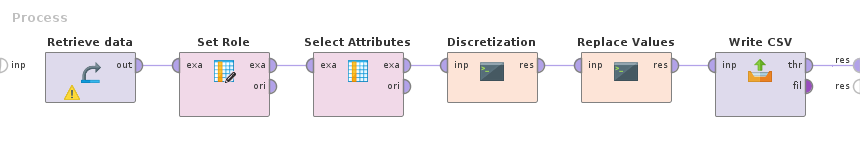
\includegraphics[width=1\textwidth]{images/rapidminer-process}
		\caption{Hauptprocess}
		\label{fig:recherche:rapidminer:1:1}
	\end{subfigure} \\
	\begin{subfigure}[t]{0.5\textwidth}
		\centering
		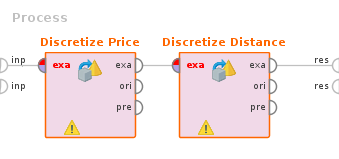
\includegraphics[width=1\textwidth]{images/rapidminer-process-discretization}
		\caption{Subprocess für die Diskretisierung}
		\label{fig:recherche:rapidminer:1:2}
	\end{subfigure}
	\begin{subfigure}[t]{0.8\textwidth}
		\centering
		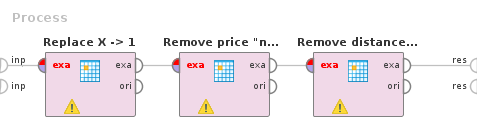
\includegraphics[width=1\textwidth]{images/rapidminer-process-replace-values}
		\caption{Subprocess für die Ersetzung von Attributwerten}
		\label{fig:recherche:rapidminer:1:3}
	\end{subfigure}
	\caption{RapidMiner Prozess für die Vorbereitung der Daten}
	\label{fig:recherche:rapidminer:1}
\end{figure}